\chapter{Numerical Examples}\label{chap6}%%% 6


\section{Introduction}\label{chap6-sec6.1}\pageoriginale%\section 6.1

We present here in some detail, a few worked-out examples showing how
the techniques discussed in the lectures are actually
employed. Unfortunately we do not show all the procedures, but it
should not be difficult for the interested reader to try out the missing
ones. We use path following via \textbf{Euler-Newton} continuation in
both the natural parameter formulation and in the Pseudoarclength
variant. Folds are circumvented by switching from the natural
parameter to Pseudoarclength when specific tests tell us to do
so. Then we switch back after the fold has been traversed. We jump
over bifurcation points easily and indeed must continuously test to
see if we must return to locate the folds or bifurcation points. We
also locate the singular points accurately and switch branches at the
bifurcation points. Multiparameter problems are also treated. 

The basic logic of our code is illustrated by a simple flow
diagram. The numerical schemes employed are given. Details of the
tests used and some indication of how they performed are given
below. Several problems have been solved and we show graphs of
solution paths for some of these problems. Some actual computer
listings of convergence data, steplength changes, accurate location of
folds and bifurcation points are included with explanation. 


\section{Problems and Difference
  Schemes}\label{chap6-sec6.2}\pageoriginale%sec  6.2 
Due to limitations of computing power available for these tests, we
consider only O.D.E. problems. They are of the form: 
\begin{equation*}
Lu \equiv \frac{d^2 u}{dx^2} + p(x) \frac{du}{dx} =
f(u,x,\lambda,\tau, \text{ in } (0,L)\tag{6.3} \label{chap6-eq6.3}
\end{equation*}
subject to two point boundary conditions of the form: 
\begin{equation*}
\begin{aligned}
& {\rm (a)} \;\;  B_0 u \equiv q_0 ~u(0) + r_0 ~\frac{du}{dx} (0) = s_0,\\
& {\rm (b)} \;\;  B_L u \equiv q_L ~u(L) + r_L ~\frac{du}{dx} (L) = s_L. 
\end{aligned}
\tag{6.4}\label{chap6-eq6.4}
\end{equation*}

The nonlinearities were of the semilinear form. No conceptual
difficulties occur if they are allowed to be quasilinear, i.e. $f$ is
in the form $f\left(u,\dfrac{du}{dx},x,\lambda,\tau \right)$. We use
uniform grids of spacing 
\begin{equation*}
h = \frac{L}{N}, \tag{6.5a}\label{chap6-eq6.5a}
\end{equation*}
to define the netpoints $\{ x_j\}^N_0$ as :
\begin{equation*}
x_0  = 0,x_{j+1} = x_j + h, j= 0,1,\ldots N-1.\tag{6.5b}\label{chap6-eq6.5b}
\end{equation*}

The usual centred difference scheme is employed, sometimes modified if
singular coefficients occur $\left(\text{i.e. } : p(x) =
  \dfrac{m}{\alpha} \right)$ or improved to get fourth order accuracy
  if $p(x) = 0$. If either $r_0 \neq 0 $ or $r_L \neq 0$, we introduce
  exterior points at $x_{-1 = -h}$ and $x_{N+1} = L+h$
  respectively. Denoting the discrete approximation to $u(x_j)$ by
  $u_j$ and using the finite difference operators:  
$$
D_+ u_j \equiv \frac{u_{j+1}-u_j}{h} ; D_{-u_j}\equiv \frac{u_j
  -u_{j-1}}{h} ; D_0 u_j \equiv \frac{u_{j+1}-u_{j-1}}{h}. 
$$

Our\pageoriginale basic difference approximation to
\eqref{chap6-eq6.3} at $x_j$ is given by:  
\begin{equation*}
L_hu_j \equiv D_+ D_-u_j +p(x) D_0u_j = f(u_j,x_j,\lambda,\tau); j =
0,1,\ldots N.\tag{6.6}\label{chap6-eq6.6} 
\end{equation*}

The boundary conditions \eqref{chap6-eq6.4} are approximated as:
\begin{align*}
\begin{split}
&\text{(a)}~ B^h_0 u_L \equiv q_0 u_0 + r_0 D_0 u_0 = s_0,\\ 
&\text{(b)}~ B^h_L u_L \equiv q_L u_N + r_L D_0 u_N = s_L,
\end{split}\tag{6.7}\label{chap6-eq6.7}
\end{align*}

The scheme in \eqref{chap6-eq6.6} for $j = 0$ and (\ref{chap6-eq6.7}a)
both involve 
$u_{-1}$. This quantity is then eliminated using the two equations to
get one relation between $u_0$ and $u_1$. A similar treatment using
\eqref{chap6-eq6.6} at $j=N$ and (\ref{chap6-eq6.7}b) eliminates
$u_{N+1}$ and retains one 
equation in $u_N$ and $u_{N-1}$. The system thus reduced consists of
$N+1$ equations in as many unknowns $u_j$, $j = 0,\ldots N$. If  $r_0 =
0$ and (or) $r_L = 0$, we do not impose \eqref{chap6-eq6.6} for $j=0$
and (or) $j = N$. The corresponding elimination need not be done and
we again get 
$N+1$ equations in the same number of unknowns. We could also
eliminate $u_0$ and (or) $u_N$. In this case we not bother to do that
in our description here. 

The difference scheme in \eqref{chap6-eq6.6}, \eqref{chap6-eq6.7} has
second order accuracy. If 
the continuous problem \eqref{chap6-eq6.3}, \eqref{chap6-eq6.4} has an
isolated solution $U_0$ 
(say, for fixed $\lambda,\tau$) and if $p(x)$ and $f$ are smooth,
then it is known that, for sufficiently small $h$, the discrete
problem \eqref{chap6-eq6.6}, \eqref{chap6-eq6.7} has a unique solution
$\{ u_j\}$ in some sphere 
in $R^{N+1}$ about $\{u_0(x_j)\}$ and further it satisfies: 
$$
|| u_0 (x_j)-u_j || = 0(h^2).
$$

Similar\pageoriginale results also apply to the entire solution branches of
\eqref{chap6-eq6.3}, \eqref{chap6-eq6.4} containing simple fold and
bifurcation points. However 
there may be some degradation of accuracy at these special points;
this is discussed more thoroughly in the expanded version of these
notes. 

If $p(x) \equiv 0$, we can easily get fourth order accurate, three point
schemes, using Collatz's device as follows. Taylor expansions give: 
$$
D_+D_-u(x_j) = \frac{d^2 u}{dx^2}(x_j) + \frac{h^2}{12}  
\frac{d^4u}{dx^4}(x_j) + 0(h^4). 
$$

Since $u(x)$ satisfies:
$$
\frac{d^2 u}{dx^2} = f(u(x),x,\lambda,\tau), 
$$
we have:
$$
D_+D_-f(u(x_j),x_j\lambda,\tau) = \frac{d^4 u}{dx^4}(x_j) + 0(h^2), 
$$
and thus we get:
$$
D_+D_- u(x_j) - \frac{h^2}{12} D_+ D_- f(u(x_j),x_j,\lambda,\tau) =
\frac{d^2 u}{dx^2}(x_j) + 0(h^4). 
$$

Thus in place of \eqref{chap6-eq6.6} we use, when $p(x) \equiv 0$ : 
\begin{equation*}
L_h u_j \equiv D_+ D_- u_j - \frac{1}{12}(f_{j+1} + 10f_j + f_{j-1}), j=
0,1,\ldots N.\tag{6.8} \label{chap6-eq6.8}
\end{equation*}

Here we have used the abbreviations:
$$
f_j \equiv f(u_j,x_j,\lambda,\tau). 
$$

We can employ this device even when we have the mixed boundary
conditions \eqref{chap6-eq6.4}. That is even when $r_0 \neq 0$ and
(or) $r_L \neq 0$. This does not\pageoriginale seem to have been
stressed before, so we indicate 
the details. Again Taylor expansions give: 
$$
D_0u(x_j) = \frac{du}{dx} (x_j)  + \frac{h^2}{12} \frac{d^3 u}{dx^3}
(x_j) + 0(h^4). 
$$

Here the factor $h^2/12$ occurs because we use $D_0$ to approximate
$d/dx$ and  $2.3! = 12$. Previously this factor came $4!/2$. In any
event now 
$$
D_0 \frac{d^2 u}{dx^2}(x_j) = \frac{d^3 u(x_j)}{dx^3} + 0(h^3). 
$$

Using \eqref{chap6-eq6.3} with $p(x) \equiv 0$ at $x = x_j$, in the
above, we get 
$$
D_0 u(x_j) - \frac{h^2}{12} D_0 f(u(x_j),x_j,\lambda,\tau) =
\frac{du}{dx}(x_j) + 0(h^2). 
$$

With $x_j = x_0$, and $x_j = x_N$, we replace \eqref{chap6-eq6.7} by : 
\begin{equation*}
\begin{split}
{\rm  (a)}~ \tilde{B}_0^h u_0 \equiv q_0 u_0 + r_0 D_0 (u_0 -
  \frac{h^2}{12} f_0) = s_0,\\ 
{\rm (b)}~ \quad \tilde{B}_L^h u_N \equiv q_L u_N + q_L u_N + r_L D_0 (u_N
  - \frac{h^2}{12} f_N) = s_L,
\end{split}\tag{6.9} \label{chap6-eq6.9}
\end{equation*}

Now (\ref{chap6-eq6.9}a) and \eqref{chap6-eq6.8}, for $j = 0$, both
contain non-zero multiples 
of $(u_{-1}-\dfrac{h^2}{12} f_{-1})$ which can be eliminated between
these two equations. A similar treatment with (\ref{chap6-eq6.9}b) and
\eqref{chap6-eq6.8} for
$j = N$ eliminates $(u_{N+1} - \dfrac{h^2}{12}f_{N+1})$. The result is
again $N+1$ equations in the basic unknowns $u_j$, $j = 0,1,\ldots N$ and
the tridiagonal structure of the system is retained [see the equation
  (6.10) below]. Of course if $r_0 = 0$ and (or) $r_L =
0$, we need 
not bother with the above procedure at $j = 0$ and (or) $j = n$. So in
either of those cases, we need not impose \eqref{chap6-eq6.8} for $j
=0$ and (or) $j = N$ respectively. Even if the elimination of $(u_{-1} -
\dfrac{h^2}{12}f_{-1})$ etc. are not performed we get enhanced
accuracy, but the system\pageoriginale structure is not as elegant. 

In the case of singular coefficients, (i.e: $p(x)
=\dfrac{m}{x^{\alpha}}, 0<\alpha \leq 1)$ we modify the scheme as
follows. For $j = 0 $ we replace \eqref{chap6-eq6.6} by:  
$$
(m+1) D_+ D_- u_0 = f_0, \text{ if } \alpha = 1,  
$$
and  
$$
D_+D_- u_0 = f_0 \text{ if } 0< \alpha < 1.
$$

These follow from $u_x(0) = 0$ and hence : 
\begin{equation*}
\lim_{x\rightarrow 0} (u_{xx} + \frac{m}{x^\alpha} u_x) =
\begin{cases}
(m+1)u_{xx}(0), \quad \text{if} \quad \alpha = 1,\\
u_{xx}(0), \quad \text{if} \quad  0 < \alpha < 1.
\end{cases}
\end{equation*}

We get only second order accuracy but the error expansion at $x=0$
proceeds in power of $h^2$. 

All the difference schemes we have described can now be incorporated
into the general form: 
\begin{align*}
g_j(u_{j-1},u_j,u_{j+1},\lambda,\tau ) & \equiv \alpha_j u_{j-1} +
\beta_j u_j + \gamma_j u_{j+1}-\hat{\alpha}_jf_{j-1}\\
& \quad -\hat{\beta}_j
f_{j}-\hat{\gamma}_j f_{j+1} -\delta_j = 0, 0 \leq j \leq
N.\tag{6.10a} \label{chap6-eq6.10a} 
\end{align*}

Of course we always have :
\begin{equation*}
\alpha_0 = \hat{\alpha}_0 = \gamma_N = \hat{\gamma}_N = 0,\tag{6.10b}
\label{chap6-eq6.10b} 
\end{equation*}
and hence :
\begin{equation*}
g_0 \equiv g_0 (u_0,u_1,\lambda,\tau) ; g_N \equiv
g_N(u_{N-1},u_N,\lambda,\tau).\tag{6.10c} \label{chap6-eq6.10c}
\end{equation*}

The system (6.10) is our finite dimensional problem which we can
write in the\pageoriginale vector form: 
\begin{equation*}
G(u,\lambda,\tau) = 
\begin{bmatrix}
g_0\\
g_1\\
\vdots\\
g_N\\
\end{bmatrix}
= 0 .
\end{equation*}

Thus our general finite dimensional problem is from $\mathbb{R}^{N+3}$
to $\mathbb{R}^{N+1}$. Note that it is a nonlinear three term
recursion, terminated at $j = 0$ and $j = N$ with two term relations. 

Of paramount importance are the derivatives of $G$ with respect to
$u$, $\lambda$ and $\tau$. The $j^{\rm th}$ row of the Jacobian matrix $G_u$ is
given by the $N+1$ vector: 
$$
\frac{\partial g_i}{\partial \underset{\sim}{u}} = (0,\ldots
0,a_j,b_j,c_j,0,\ldots 0), j = 0, \ldots N. 
$$

Thus $G_u$ is a tridiagonal matrix with $b_j$ on the diagonal, $a_j$
and $c_j$ are below and above the diagonal respectively. In standard
notations for such matrices we have:  
\begin{equation*}
G_u(u,\lambda,\tau ) \equiv [a_j,b_j,c_j]^N_0.\tag{6.11}\label{chap6-eq6.11}
\end{equation*}

Differentiating \eqref{chap6-eq6.10a} we get that :
\begin{equation*}
\begin{split}
& a_j \equiv \frac{\partial g_j}{\partial u_{j-1}} = \alpha_j -
  \hat{\alpha}_j (f_u)_{j-1},\\ 
& b_j \equiv \frac{\partial g_j}{\partial u_j} ~~~= \beta_j -
  \hat{\beta}_j (f_u)_j,\\ 
& c_j \equiv \frac{\partial g_j}{\partial u_{j+1}} = \gamma_j -
  \hat{\gamma}_j(f_u)_{j+1}, 0 \leq j \leq N.
\end{split}\tag{6.12} \label{chap6-eq6.12}
\end{equation*}

The\pageoriginale tridiagonal form of \eqref{chap6-eq6.11} becomes
clear from 
\eqref{chap6-eq6.10b}\break and
\eqref{chap6-eq6.12}. Here we use the obvious notation : 
$$
(f_u)_j = \frac{\partial f}{\partial u} (u_j,x_j,\lambda, \tau ).
$$

The $\lambda$ and $\tau$ derivatives are not sparse; we have : 
\begin{equation*}
G_{\lambda} =
\begin{bmatrix}
\vdots\\
g_{\lambda,j}\\
\vdots\\
\end{bmatrix}
, \tag{6.13}\label{chap6-eq6.13}
\end{equation*}
where,
$$ 
g_{\lambda,j} = -\hat{\alpha}_j(f_\lambda)_{j-1}
-\hat{\beta}_j(f_\lambda)_j - \hat{\gamma}_j (f_\lambda)_{j+1}, 0 \leq
j \leq N. 
$$

A similar set of relations define $G_\tau$.

To complete the detailed specification of any of our problems, we need
only to give: 
\begin{equation*}
L,p(x), \; f(u,x,\lambda, \tau ), \; (q_0,r_0,s_0), \;
(q_L,r_L,s_L).\tag{6.14}\label{chap6-eq6.14} 
\end{equation*}

When these are given, we examine $p(x)$, $r_0$ and $r_L$ to find out
which of the schemes we have described is to be employed. Then the
constants 
\begin{equation*}
(\alpha_j, \beta_j, \gamma_j, \hat{\alpha}_j, \hat{\beta}_j,
  \hat{\gamma}_j, \delta_j), \quad 0 \leq j \leq N
  \tag{6.15} \label{chap6-eq6.15} 
\end{equation*}
are determined. Now only the net spacing or integer $N$ of \eqref{chap6-eq6.5a}
need be given. We give the coefficients of \eqref{chap6-eq6.15} in
table I for some of the most\pageoriginale basic cases to be tested. 


\setcounter{section}{15}
\section{Algorithm and Tests}\label{chap6-sec6.16}%sec 6.16

The following are the main steps for computing the solution branch
starting from a known initial solution $(u^o,\lambda^o)$. 

\medskip
\noindent{\textbf{Step I.}}
Determination of the unit tangent to the path, viz $\pm (\dot{u},
\dot{\lambda})$ 

\medskip
\noindent{\textbf{Step II.}}
Choice of :
\begin{enumerate}[(i)]
\item the tangent direction;

\item steplength $\triangle$, along the path;

\item continuation method; natural parameter $(n \cdot p)$ or
  pseudoarclength $(p \cdot a)$. 
\end{enumerate}

\medskip
\noindent{\textbf{Step III.}}
Construction of the initial iterate :
either for $(n \cdot p)$ : 
$$
u^{(1)} = u^o + \triangle u ;
$$
or for $(p \cdot a)$ :
\begin{align*}
 u^{(1)} & = u^o + \triangle \dot{u},\\
 \lambda^{(1)} & = \lambda^o + \triangle \dot{\lambda}
\end{align*}

\medskip
\noindent{\textbf{Step IV.}}
Newton's iteration to find $(\delta u)$ of $(\delta u, \delta
\lambda)$. 

\medskip
\noindent{\textbf{Step V.}}
Computation of the relation error;

If error $< \varepsilon$, then one step is completed and then go to
Step $I$ to determine the next solution. If not, then update $(u)$ or
$(u,\lambda)$ and go to Step IV.

The steps in the algorithm are explained in more detail in the
flow\-chart.\pageoriginale No we explain step II, where certain tests are used to
make the various choices mentioned. 

The unit tangent $(\dot{u}, \dot{\lambda})$ is determined only up to
its sign. The choice of the sign is crucial in order to avoid going
backwards or getting trapped between two points. If the tangent at the
previous solution is $(\dot{u}^o, \dot{\lambda}^o)$ then we choose the
sign for $( \dot{u}, \dot{\lambda})$, so as to make the inner product $\langle 
( \dot{u}^o, \dot{\lambda}^o),( \dot{u}, \dot{\lambda})\rangle$ positive.  

The choice of the steplength is more delicate as it depends upon a
number of parameters. If the steplength is too large, we may require
too many Newton iterations to converge (or indeed divergence can
occur). It the steplength is too small we may require too many steps
to compute the entire solution path. Thus in either case the
computational efficiency is reduced. At each point on the branch, we
allow the steplength $\triangle$, to vary with $U_F$, the number of
iterations required to converge at the previous step. We fit a
decreasing exponential curve in the $(\triangle,U)$-plane and choose
$\triangle$ according to this function. Specifically, we use 
$$
\triangle_{\text new} = \theta(U_F) \triangle_{\text old}, 
$$
where
$$
\theta(U) \equiv 2^{ \left(\frac{4-U}{3} \right)}.
$$

Naturally other choices for $\theta(U)$ can be used. 
 
The choice of the method depends on whether we are near a
singular\pageoriginale 
point or not. Most often we can pass over simple bifurcation points
even with natural parameter continuation. Thus the difficulty arises
mainly near the folds. Since $\dot{\lambda} = 0$ at the fold, it seems
reasonable to switch over to pseudoarclength continuation when
$|\dot{\lambda} |$ is small enough. Once the fold is crossed over,
$|\dot{\lambda} |$ increases again and we switch back using the same
test. 

In pseudoarclength continuation, two different types of bordering
algorithm can be used depending on whether the matrix $G_u$ is nearly
singular or not. To do this we need a test to determine if $G_u$ is
``sufficiently'' singular. For that we look at the $LU$ decomposition
for $G_u$ and test the diagonal elements, $u_{j,j}$, of $U$ as follows: 
$$
\underset{1\leq j\leq N-1}{Min} \quad \left|
\frac{u_{j,j}}{u_{j-1,j-1}} \right| > M \left|
\frac{u_{NN}}{u_{N-1,N-1}} \right|, 
$$
where $M$ is a constant depending on the number of points $N$. If the
test is passed, we can use the bordering algorithm in the singular
case. Otherwise the usual bordering algorithm is used. In most
computations, however, the singular bordering algorithm is invoked
only when great accuracy is sought. 


\section{Numerical Examples}\label{chap6-sec6.17}%sec 6.17

The algorithm was used to compute the solution branches for simple
nonlinearities in double precision with an error tolerance of
1.E-8.

\setcounter{exam}{0} 
\begin{exam}\label{chap6-exam1}
We consider the following nonlinear O.D.E.
\begin{equation*}
\begin{split}
& u_{rr}+\frac{(n-1)u_r}{r}+u^3+\lambda =0 \text{ in } ( 0, 1),\\ 
& u'(0)=0; u(1) = 0, n\ge 2
\end{split}\tag{6.18}\label{chap6-eq6.18}
\end{equation*}\pageoriginale

A difference scheme, as described in the earlier section was used with
twenty points. The coefficients are as listed in case (5) of
table-I, with the additional assumption $s_L = 0$ and $q_L
=1$. Starting from the trivial solution at $\lambda =0$, the branch was
computed beyond two folds. Table II gives the convergence data for
the first few steps. Notice that near the turning point,
pseudoarclength continuation is opted for but later natural parameter
continuation. The sign of the determinant  changes indicating the
crossing of a singular point, a turning point in this
case. Fig.~\ref{chap6-fig6.1} plots, for $n=2$, norm $u=(\sqrt{\mid u'
  (1)u(0)\mid}) \text{\,sgn\,}(-u' (1))$ versus $\lambda $, showing
the two folds.  

After a certain number of iterations, the continuation is stopped and
the program proceeds to the location of singular points. Starting from
the stored value of $(u,\lambda)$, just before the determinant changed
sign, using a bisection method, the fold is located accurately. In the
vicinity of the fold, the singular bordering algorithm (refer section,
\ref{chap4-sec4.11}, for the case of almost singular A) is used and the method
converges well. Table III gives the convergence pattern near the
first fold for $n=2$. 
\end{exam}

\begin{exam}\label{chap6-exam2}%exam 2
 Here we consider a two parameter problem: 
\begin{equation*}
\begin{split}
 -u'' & = u^2-\lambda u+\mu  \quad \text{in}(0,1)\\
  u(0) & = u(1)=0
\end{split}\tag{6.19}\label{chap6-eq6.19}
\end{equation*}

For\pageoriginale $\mu =0$, the simple bifurcation points along the
trivial branch 
$u\equiv 0$ are at $\lambda =\lambda _j$ where $\lambda _j$ are the
eigenvalues of $\{-\dfrac{d^2}{dx^2}\}$ on $(0,1)$.  We use the
perturbed bifurcation approach, (Method V in section \ref{chap5-sec5.26} of
chapter \ref{chap5}) to get the branch bifurcating from the trivial branch at
$\lambda _1$. Here we use $\mu$ to perturb the problem (refer
\eqref{chap5-eq5.33} 
where $\tau _q$ was used in a similar role.) In
fig.~\ref{chap6-fig6.2}, we plot 
norm $u=(\sqrt {u_{\max}}) \text { sgn }(u'(0)) \text{ versus
}\lambda$. The difference scheme used is an in case 1 of table - I
with $N=20$.  

Starting from
$$
(u,\lambda, \mu )=(0,0,0).
$$
continuation in $\mu$ is done up to $\mu=\varepsilon$, keeping $\lambda$
fixed at 0. Then keeping $\mu =\varepsilon$, fixed, a $\lambda$
continuation is done till the solutions are sufficiently large. These
solutions are indicated in Fig.~\ref{chap6-fig6.2} by two solid lines: upper one
for $\mu=.1$ and lower on for $\mu=-.1$. Now to switch from $\mu =
\varepsilon$ back to $\mu=0$, we do a $\mu$-continuation. Then keeping
$\mu=0$ fixed, continuing in $\lambda$, we get the branch bifurcating
from $(0,\lambda_1)$. This branch is indicated by the dotted line in
Fig.~\ref{chap6-fig6.2}. 
\end{exam}

\begin{exam}\label{chap6-exam3}%\exa 3
The following nonlinear ODE is the one dimensional version of
\eqref{chap6-eq6.18} (i.e. $n=1$) : 
\begin{equation*}
\begin{split}
& u''+u^3+\lambda =0 \text{ in }(0,1)\\
&u(0)=u(1)=0 
\end{split}\tag{6.20}\label{chap6-eq6.20}
\end{equation*}

Starting from the trivial solution $(u, \lambda)=(0,0)$, the branch is
continued till $\mid \lambda \mid\ge 16$. Two singular points are
found and they are located accurately\pageoriginale at $\lambda \simeq 1.1$ and
$\lambda \simeq - 8.07$ using a bisection method as in example-1
Table-IV shows the Patten near the second singular point.   
\end{exam}

Once a good approximation to the singular point is obtained, the right
and left null vectors $\Phi$  and $\psi $ of $G_u$ are computed as
indicated in Chapter IV. At the first singular point , $<\psi$,
$G_\lambda > \simeq 120$. This shows that is must be a fold point. At
the second singular point where $\lambda \simeq -8.10$, we find that
$<\psi$, $G_\lambda >\simeq 1.E-4$. (See table-IV and also the remark
after lemma (\ref{chap5-lem5.20}) in chapter \ref{chap5}). This is
indeed a bifurcation 
point. The branch switching is done using method II of Chapter \ref{chap5},
taking care to use a large step size. This gives one part of the
second branch. Reversing the direction, we get the other part of the
second branch, bifurcating from the original one. 

The bifurcating diagram is given in Fig.~\ref{chap6-fig6.3}. Here norm
$u$ actually 
stands for $(sgn u' (0))u_{\max}$. The branch I represents symmetric
solution which are positive till the bifurcating point. After the
bifurcation point, the branch develops two nodes near each end. The
branch II represents non-symmetric solutions bifurcating from branch
I. The solutions in the upper branch have a node near the right end
and those in the lower branch near the left end. 


{\fontsize{9}{11}\selectfont
\begin{center}
\textbf{Table - 1}\pageoriginale

\medskip
\renewcommand{\arraystretch}{1.6}
\tabcolsep=1.6pt
\begin{tabular}{cccccccc}
\hline
&Case~(1) & Case~(2) & Case~(3) & Case~(4) & Case~(5)\\
\hline
& $p(x)\equiv 0$ & $p(x)\not\equiv0$  & $p(x)\equiv 0$ &
$p(x)\not\equiv 0$ & $p(x)=\dfrac{m}{x}$\\ 
&$r_0=0=r_L$ & $r_0=0=r_L$ & $r_0\neq 0, r_L \neq 0$ & $ r_0\neq 0,
r_L \neq 0$ & $r_0=1,s_0=0$\\
& & & & & $ q_o = 0 = r_L$\\ 
& 4th order & 2nd order& 4th order & 2nd order & 2nd order\\
& accuracy & accuracy& accuracy & accuracy & accuracy \\ 
\hline
& & & & & & \\[-0.4cm]
 $\beta_0 $ & $q_o$ & $q_0$ & $-\dfrac{2}{h^2}+\dfrac{2q_0}{r_0 h}$ &
$-\dfrac{2}{h^2}+\dfrac{2q_0}{r_0h}-\dfrac{p_0q_0}{r_0}$ &
$-\dfrac{2}{h^2}(m+1)$\\[8pt]  
  $\gamma_0$ & $0$ & $0$ & $\dfrac{2}{h^2}$ & $\dfrac{2}{h^2}$ &
$\dfrac{2}{h^2}(m+1)$ \\[5pt] 
 \hline
 $\hat{\beta}_0$ & $0$ & $0$ & $5/6$ & $1$ & $1$\\
 $\hat{\gamma}$ & $0$ & $0$ & $1/6$ & $0$ & $0$\\
 $\delta_0$ & $s_0$ & $s_0$ & $\dfrac{2s_0}{r_0h}$ &
 $\dfrac{s_0}{r_0}(\dfrac{2}{h}-p_0)$ & $0$\\ 
 \hline
& & & & & & \\[-0.4cm]
 $\alpha_j$ & $1/h^2$ & $1/h^2 -p_j /2h$ &$1/h^2$&
 $\dfrac{1}{h^2}-\dfrac{p_j}{2h} $ & $\dfrac{1}{h^2}-
 \dfrac{m}{2jh^2}$\\ 
  $\beta_j$ & $-2/h^2$ & $-2/h^2$& $-2/h^2$& $-2/h^2$& $-2/h^2$\\ 
  $\gamma_j$ & $1/h^2$ &  $1/h^2 + p_j /2h$ & $1/h^2$ & $1/h^2 +p_j
 /2h$ & $1/h^2 + m /2jh^2$\\[5pt]
 \hline
 $\hat{\alpha}_j$ & $1/12$ & $0$ & $1/12$ & $0$ & $0$\\
  $\hat{\beta}_j$ & $5/6$ & $1$ & $5/6$ & $1$ & $1$\\
 $\hat{\gamma}_j$ & $1/12$ & $0$ & $1/12$ & $0$ & $0$\\
\hline
$\alpha_N$ & $0$ & $0$ & $2/h^2$ & $2/h^2$ & $2/h^2$  \\
$\beta_N$ & $q_L$ & $q_L$ & $- \dfrac{2}{h^2}- \dfrac{2q_L}{r_Lh}$ &
$- \dfrac{2}{h^2} - \dfrac{2q_L}{r_Lh} - \dfrac{p_Nq_L}{r_L}$ & \;\;$-
\dfrac{2}{h^2}- \dfrac{q_L}{r_L}(\dfrac{1}{h}+ m)$\\[6pt] 
\hline
$\hat{\alpha}_N$ & $0$ & $0$ & $1/6$ & $0$ & $0$\\
$\hat{\beta}_N$ & $0$ & $0$ & $5/6$ & $1$ & $1$\\
$\delta _N$  & $s_L$ & $s_L$ & $-\dfrac{2s_L}{r_Lh}$ &
$-\dfrac{s_L}{r_L}(\dfrac{2}{h}+P_N)$ & $s_L$\\[6pt] 
\hline
\end{tabular}
\end{center}}\relax

\begin{center}
\textbf{\Large Flow Chart}\pageoriginale
\end{center}
\vskip -1cm
\begin{figure}[H]
\centering
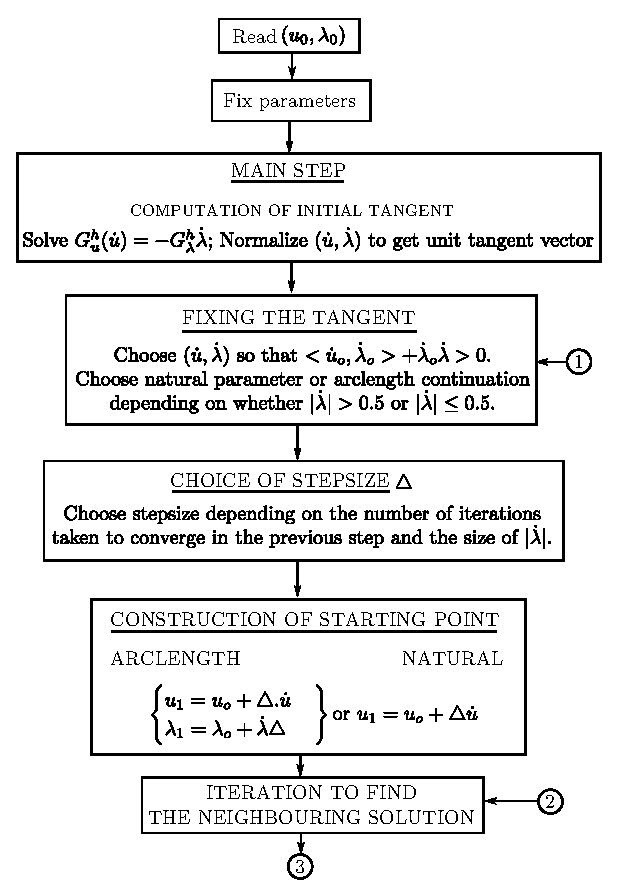
\includegraphics[scale=1]{vol79-fig/fig79-flowchart1.eps}
\end{figure}

%%%%

\bigskip


\begin{figure}[H]
\centering
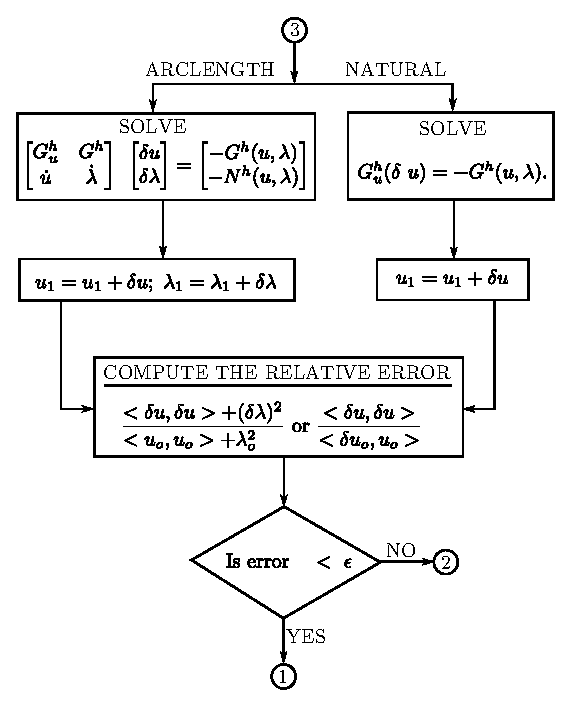
\includegraphics[scale=1.2]{vol79-fig/fig79-flowchart2.eps}
\end{figure}\pageoriginale

\vfill\eject

{\fontsize{8}{10}\selectfont
\begin{center}
{\bf TABLE - II}\pageoriginale
\medskip
\renewcommand{\arraystretch}{2}
\tabcolsep=2pt
\begin{tabular}{cccccccc}
\hline
 MAIN  & METHOD & ITERATION & STEPLENGTH  &  ERROR & $\lambda$ & SIGN
 OF THE  \\ 
 STEP & USED & &  $\Delta$ & & OBTAINED & DETERMINANT\\
  \hline
 $1$ & (p.a) & $1$ & & .$3E-3$ \\ 
 &  & & $0.5$ & & $0.23$ & $+1$\\
  & nonsingular & $2$ & & .$3E-10$ & & \\
  \hline 
  $2$ & (p.a)  & $1$ & & .$1E-1$\\
  & nonsingular & $2$ & $0.794$ & .$2E-5$ & $0.45$ & $+1$\\
  & & $3$ & & .$5E-13$ \\
  \hline
  $3$ & (p.a) & $1$ & & .$5E-3$\\
  & nonsingular & $2$ & $1.0$ & .$2E-3$ & $0.003$ & $-1$\\
  & & $3$ & & .$9E-11$\\
  \hline 
  $4$ & & $1$  & & .$5E-1$\\
  & &  $2$ & & .$5E-2$\\
  &  (n.p) & &  $1.357$ & & $-1.35$  & $-1$\\
  & & $3$ &   & .$2E-4$ \\
  & &  $4$ & & .$2E-8$ \\
  \hline 
  $5$ & & $1$ & & .$1E-1$\\
  & & $2$ & & .$8E-4$ \\
  & (n.p) & & $1.357$  &  & $-2.71$ & $-1$\\
  & & $3$ & &  .$1E-7$\\
  & & $4$ & & .$5E-15$ \\         
\hline
  \end{tabular}
\end{center}}\relax

\vfill\eject

{\fontsize{8}{10}\selectfont
  \begin{center}
{\bf TABLE - III}\pageoriginale

\medskip
\renewcommand{\arraystretch}{1.4}
\tabcolsep=2pt
\begin{tabular}{ccccccc}
\hline
MAIN & BORDERING  & ITERATION & ERROR & $\lambda$ &  LAST &  SING OF THE \\
STEP & ALGORITHM & & & OBTAINED & PIVOT & DETERMINANT \\
& TYPE \\ 
\hline
1 & NS & 1 & .2E-4 \\
& & & & 0.45085 & $-462.1$ & $-1$ \\
& (nonsingular) & 2 & .$1E-11$ \\
\hline
2 & NS & 1 & .$1E-5$ \\
& & & & $0.45275$ & $66.8$ & $+1$ \\
& & 2 & .$4E-14$ \\
\hline
3 & NS & 1 & .$9E-9$ \\
& & & & $0.452495$ & $-164.8$ & $-1$ \\
& & 2 & .$2E-16$ \\
\hline
4 & NS & 1 & .$4E-6$\\
& & & & 0.452721 & $-84.73$ & $-1$ \\
& & 2 & .$4E-15$ \\
\hline
5 & NS & 1 & .$8E-6$ \\
& & & & 0.45276 & $-22.79$ & $-1$ \\
& & 2 & .$2E-14$ \\
\hline
6 & NS & 1 & .$1E-5$ \\
& & & & 0.452761 & 17.51 & $+1$ \\
& & 2 & .$2E-14$ \\
\hline
7 & S & 1 & .$9E-6$ \\
& & & & 0.452762 & $- 3.6$ & $-1$ \\
& (singular)& 2 & .$5E-12$ \\
\hline
8 & S & 1 & .$1E-5$ \\
& & & & 0.452762 & 6.7 & $+1$ \\
& & 2 & .$2E-11$ \\
\hline
9 & S & 1 & .$1E-5$ \\
& & & & 0.452762 & 1.485 & $+ 1$ \\
\hline
10 & S & 1 & .$1E-5$ \\
& & & & 0.452762 & $-1.073$ & $-1$ \\
& & 2 & .$4E-13$ \\
\hline
\end{tabular}
  \end{center}}\relax

\vfill\eject

{\fontsize{9}{11}\selectfont
\begin{center}
{\bf TABLE - IV}\pageoriginale

\medskip
\renewcommand{\arraystretch}{1.7}
\tabcolsep=2pt
\begin{tabular}{ccccccc}
\hline
MAIN & ITERATION & ERROR & $\lambda$ &  LAST &  SING OF THE & $< \Psi,
G_\lambda >$ \\ 
STEP  & & & OBTAINED & PIVOT & DETERMINANT \\
\hline
1 & 1 & .$1E-4$ \\
& 2 & .$2E-8$ & $-8.643$ & $-31.9$ & $-1$ & $-2.3$\\[4pt]
2 & 1 & .$1E-5$ \\
& 2 & .$8E-11$ & $-8.223$ & $-8.4$ & $-1$ & $-.5$\\[4pt]
3 & 1 & .$8E-7$ \\
& 2 & .$5E-13$ & $-8.014$ & $-3.7$ & $+1$ & $-.26$\\[4pt]
4 & 1 & .$3E-6$ \\
& 2 & .$8E-12$ & $-8.118$ & $-2.4$ & $-1$ & $-.17$\\[4pt]
5 & 1 & .$1E-6$ \\
& 2 & .$2E-12$ & $-8.066$ & $-67$ & $+1$ & $-.047$\\[4pt]
6 & 1 & .$2E-6$ \\
& 2 & .$4E-12$ & $-8.092$ & $-.86$ & $-1$ & $-.061$\\[4pt]
7 & 1 & .$2E-6$ \\
& 2 & .$3E-12$ & $-8.0792$ & $-.096$ & $-1$ & $-.0068$\\[4pt]
8 & 1 & .$2E-6$ \\
& 2 & .$3E-12$ & $-8.0727$ & $-.284$ & $+1$ & $-.02$\\[4pt]
9 & 1 & .$2E-6$ \\
& 2 & .$3E-12$ & $-8.076$ & $-.094$ & $+1$ & $-.0067$\\[4pt]
10 & 1 & .$2E-6$ \\
& 2 & .$3E-12$ & $-8.07759$ & $-.001$ & $-1$ & $-.00008$\\
\hline
\end{tabular} 
\end{center}}\relax

\vfill\eject

\begin{figure}[H]
\centering
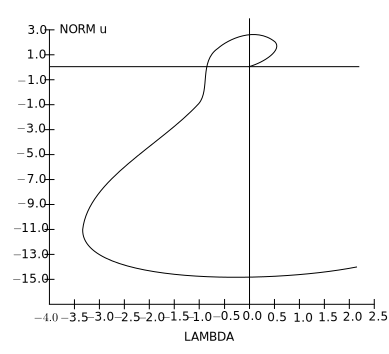
\includegraphics[scale=0.75]{vol79-fig/fig79-31.eps}
\smallskip
\caption{}\label{chap6-fig6.1}
\end{figure}\pageoriginale
%%
\begin{figure}[H]
\centering
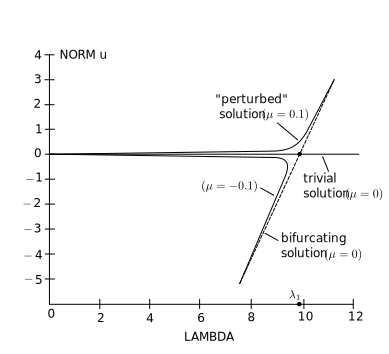
\includegraphics[scale=0.85]{vol79-fig/fig79-32.eps}
\smallskip
\caption{}\label{chap6-fig6.2}
\end{figure}\pageoriginale

\begin{figure}[H]
\centering
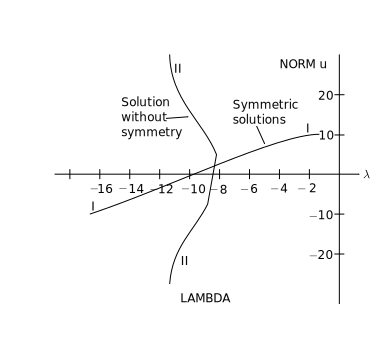
\includegraphics{vol79-fig/fig79-33.eps}
\smallskip
\caption{}\label{chap6-fig6.3}
\end{figure}\pageoriginale

\def\referencename{References}
\def\bibname{References}

\begin{thebibliography}{99} 
\bibitem{key1} {P. ABRAHAM and J. ROBBIN} Transversal mapping and flows,
  Benjamin Press, New York, 1967. 

\bibitem{key2} {F.H. BRANIN JR.,} Widely convergent method for finding
  multiple solutions of simultaneous nonlinear equations, IBM
  J. Research Develop. 16, 1972, 504 - 522. 

\bibitem {key3} {Y. M CHEN and P.L. CHRISTIANSEN,} Application of a
  modified Newton's iteration method to construct solutions of
  eigenvalue problems of nonlinear PDE, SIAM J.Num. Anal. 18,
  1970, 335 - 345. 

\bibitem {key4} {S.N. CHOW and J.K. HALE,} Methods of bifurcation theory,
  Springer Verlag, 1982. 

\bibitem {key5} {M.G. CRANDALL and P.H. PABINOWITZ,} Bifurcation from
  simple eigenvalues, J. Funct. Anal. 8, 1971, 321 - 340. 

\bibitem {key6} { D.W DECKER and H. B KELLER,} Path following near
  bifurcation, CPAM, Vol XXXIV, 1981, 149 - 175. 

\bibitem {key7} {D.W. DECKER and H.B. KELLER,} Multiple limit point
  bifurcation, J1. of Math. Anal. and Appl., Vol. 75, No. 2, June
  1980, 417 - 430. 

\bibitem {key8} {Y.M.J. DEMOULIN 	and Y.M. CHEN,} An interation method
  for solving nonlinear eigcnvalue problems, SIAM J. Appl. Math., 28,
  1975, 588 - 595. 

\bibitem {key9} {J.E. DENNIS and G.J. MORE,} Quasi Newton methods, a
  motivation and theory, SIAM Review, Vol 19, No. 1, 1977, 46-
  89. 

\bibitem {key10} {E.J. DOEDEL, A. D. JEPSON and H.B. KELLER,} Numerical
  methods for Hopf bifurcation and contiunation of periodic solution
  paths; in Computing methids in Applied Sciences and Engineering,
  IV, Ed : R. Glowinski and J.S.Lions, Elsevier Publishers,
  1984. 

\bibitem {key11} {G.F. GAUSS,} The struggle for existence, Dover
  Publications, 1964. 

\bibitem{key12} {A.H. HOUSEHOLDER,} The theory of matrices in Numerical
  Analysis, Dover Publications, 1975.

\bibitem{key13} {G. IOOSS and D. JOSEPH} Elementary stability and
  bifurcation theory, Springer Verlag, 1980. 

\bibitem{key14} {A.D JEPSON and H.B. KELLER,} Steady state and periodic
  solution paths : their birfurcations and computations ; in \textit{Numerical
  Methods for Bifuracation Problems, ISNM 70, Ed : Kupper,Mittleman,
  Weber}, Birkauser Verlag, 1984. 

\bibitem {key15} {A.D JEPSON and A. SPENCE,} Folds in solutions of two
  parameter systems and their calculations : Part I, SIAM
  J. Numer. Anal., 22, 1985, 347-368.  

\bibitem {key16} {L.V.KANTOROVICH, and G.P. AKILOV,} Functional Analysis
  in Normed Spaces, Pergamon Press, 1964. 

\bibitem {key17} {H.B. KELLER,} Practical Procedures in Path following
  Near Limit Points; in Computing methods in Applied Sciences and
  Engineering, ed: Glowinski \& Lions, North - Holland, 1982. 

\bibitem {key18} {H.B. KELLER,} Constructive methods for Bifurcation and
  Nonlinear eigenvalue problem; in Computing method in Applied
  Sciences \& Engineering, Ed : Glowinski \& Lions, Springer -
  Varlag, 1977. 

\bibitem {key19} {H.B. KELLER,} Numerical Solutions of Bifurcation and
  nonlinear eigenvalue problem; in Applications of Bifurcation Theory,
  Ed : Poul . H. Rabinowitz., Academic Press, 1977, 359-384. 

\bibitem {key20} {H.B. KELLER,} Global Homotopies and Newton methods; in
  Recent Advances in Numerical Analysis, Ed : C. De Boor and
  G.H. Golub, Academic press, 1979, 73 -94. 

\bibitem {key21} {H.B. KELLER,} Isolas and perturbed bifurcation theory;
  in Nonlinear partial differential equations in engineering and
  applied science, Ed. R.L. Sternberg, A.J Kalinowski and
  J.S. Papadakis, Marcel Dekker, 1980. 

\bibitem {key22} {H.B. KELLER and W.F. LANGFORD,} Iterations,
  pertubations and multiplicities for nonlinear bifurcation problem,
  Arch . Rat. Mech. Anal. 48, 1972, 83 - 108. 

\bibitem {key23} {H.B. KELLER, and S. ANTMANN} Bifurcation Theorey and
  Nonlinear eigenvalue problem, W.A. Benjamin, 1969. 

\bibitem {key24} {A.J. LOTKA} Elements of Mathematical Biology, Dover
  Publications 

\bibitem {key25} {MARSDEN and McCRACKEN,} Hopf bifurcation and its
  applications, Springer Verlag, 1976. 

\bibitem {key26} {L. NIRENBERG} Topics in Nonlinear Functional Analysis,
  Lecture notes, Courant Inst. MAth Sci. New - York University,
  1974. 

\bibitem {key27} {W.C. RHEINBOLDT,} Numerical Analysis of Parametrized
  nonlinear equations, J. Wiley and Sons, 1986. 

\bibitem {key28} {D.H. SATTINGER,} Topics in Stability and Bifurcation
  Theory, Lecture Notes in Mathematics, Springer Velag, 1973. 

\bibitem {key29} { J.T. SCHWARTZ,} Nolinear Functional Analysis, Gordon
  and Breach, 1969. 

\bibitem {key30} {S. SMALE,} A convergent process of price adjustment and
  global Newton Newton methods J. Math Eco. 3, 1976, 107 - 120. 

\bibitem {key31} {R.K. WEISS,} Bifurcation in difference approximations to
  two point boundary value problems, Math. of comp. 29, 1975, 746 -
  760. 

\bibitem {key32} {J.H. WILKINSON,} The Algebraic Eigenvalue Problem, 
  Oxford Uni. press 1965. 

\bibitem {key33} {ZHONG - HUA YANG and H.B. KELLER,} A direct method for
  computing order folds, SIAM J. Sci. Stat. Computing, Vol 7,
  No. 2, April 1986, 351 - 361   
\end{thebibliography}
